\chapter{KNN and Decision Tree }
This chapter will analyse the mathematics behind KNN, decision trees, and random forests as multiclass classifiers.
\begin{definition}
\textbf{Shattering} is the ability of a model to classify a set of points perfectly. More generally, the model can create a function that can divide the points into two distinct classes without overlapping. It is different from simple classification because it considers all possible combinations of labels upon those points.
\end{definition}
\begin{definition}\textbf{VC dimension}
    The Vapnik-Chervonenkis dimension, more commonly known as the VC dimension, is a model capacity measurement used in statistics and machine learning. The VC dimension of a model is the size of the largest set of points that that model can shatter.
\end{definition}

\section{KNN} KNN relies on the idea that similar data points tend to have similar labels or values. The KNN algorithm stores the entire training dataset as a reference during the training phase. When making predictions, it calculates the distance between the input data point and all the training examples, using a chosen distance metric such as Euclidean distance.

Next, the algorithm identifies the K nearest neighbours to the input data point based on their distances. In the case of classification, the algorithm assigns the most common class label among the K neighbours as the predicted label for the input data point. For regression, it calculates the average or weighted average of the target values of the K neighbours to predict the value for the input data point.


\subsection{KNN Model}

\begin{algorithm}
\caption{KNN Classification}\label{alg:knn_classification}
\begin{algorithmic}
\REQUIRE Feature matrix $X$ ($n\_samples \times n\_features$), target vector $y$ ($n\_samples$)
\ENSURE Accuracy of the KNN classifier on the test data
\STATE \textbf{Step 1: Split the Data}
    \STATE Split the data into training and testing sets using $train\_test\_split$
\STATE \textbf{Step 2: Import Libraries} import $KNeighborsClassifier$ from scikit-learn and $accuracy\_score$ from scikit-learn.metrics
\STATE \textbf{Step 3: Instantiate the KNN Classifier}
    \STATE Create an instance of $KNeighborsClassifier$ with the desired number of neighbors
\STATE \textbf{Step 4: Train the Classifier}
    \STATE Fit the classifier to the training data
\STATE \textbf{Step 5: Make Predictions}
    \STATE Use the trained classifier to predict the labels of the test data
\STATE \textbf{Step 6: Evaluate the Model}
    \STATE Calculate the accuracy of the model by comparing the predicted labels with the true labels of the test data
\STATE \textbf{Step 7: Output the Results}
    \STATE Print or return the accuracy of the model on the test data
\end{algorithmic}
\end{algorithm}
\begin{itemize}
    \item \textbf{Split data }splitting the data into training and testing sets to evaluate the model's performance is not necessary when using KNN on the same dataset.
    \item \textbf{Import libraries} import the KNeighborsClassifier from scikit-learn.
    \item Instantiate the KNN classifier: Create an instance of the KNeighborsClassifier class. Specify the number of neighbours (n\_neighbors) and other parameters.
    \item \textbf{Train classifier} Fit the classifier to your entire dataset.
    \item \textbf{Make predictions} Use the trained classifier to make predictions on the same dataset.
\end{itemize}
Since predicting on the same dataset trained on, we won't get a true evaluation of the model's performance. So, we used the trained model on a new data set to achieve accuracy.

\subsection{KNN results}
A better model was obtained by KNN with n value 5. For all input features were converted to 0 to 1 as input and target variable hot encoded. The true negative, true positive, false negative, and false positive predictions for the entirely unknown data set of around four lac data points are explained in the confusion matrix.
\begin{figure}
    \centering
    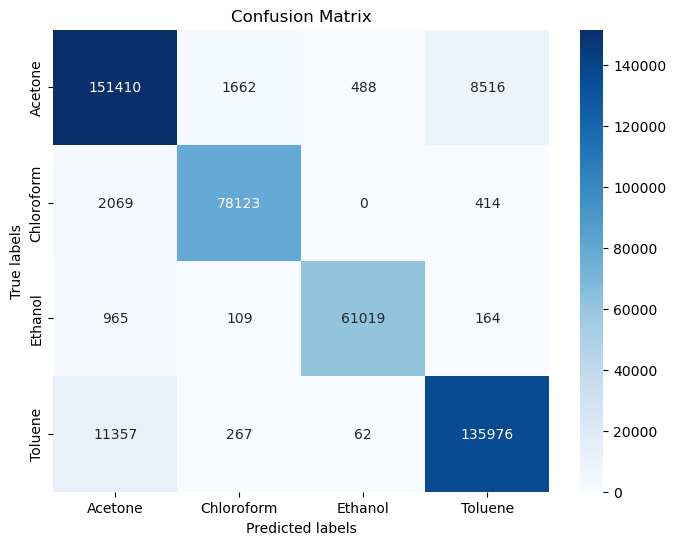
\includegraphics[width=0.8\linewidth]{Thesis Prashant//Images//Results/knn_confusion matrix.png}
    \caption{KNN Confusion Matrix}
    \label{fig:enter-label}
\end{figure}


\section{Decision Tree}

A general framework for growing a decision tree starts with a tree with a single leaf(the root) and assigns this leaf a label according to a majority vote among all labels over the training set. Then, a series of operations are performed. On each iteration, the effect of splitting a single leaf is examined. Then, among all possible splits, we choose the one that maximizes the gain and performs it or chooses not to split the leaf.

A possible Implementation is based on a popular decision tree algorithm known as "ID3" (Iterative Dichotomizer 3), 
the algorithm for the case of binary features, namely, $\xi = {0,1}_{d}$, and therefore all splitting rules are of the form $1_{[x_{i}=1]}$ for some feature $i\in [d]$.

\subsection{Analysis with Decision Tree}
Starting with splitting the data into training and testing sets to evaluate the model's performance 80\% training data and 20\% data for testing was used. Before splitting data, it is shuffled to ensure randomness. The decision tree algorithm from the library was selected and trained. And evaluated using accuracy metrics. After fine-tuning hyperparameters, the algorithm will get better accuracy. After getting the desired accuracy, the model was saved and again used for a completely new data set for cross-validation, and a new confusion matrix was used to visualize the performance of the model.
\subsubsection{hyper-parameters}
Hyperparameters in decision trees are parameters that are set before the learning process begins. They control aspects of the tree's construction and can significantly impact the resulting model's performance and behaviour. 

    \begin{itemize}
        \item \textbf{Criterion} Criterion is the function used to measure the quality of a split. Common options are "Gini" for the Gini impurity and "entropy" for information gain.
        \item \textbf{Max Depth} Max depth controls the maximum depth of the decision tree. It limits the number of nodes in the tree. Setting this parameter helps prevent overfitting.
        \item \textbf{Min Samples Split} Min samples split specifies the minimum number of samples required to split an internal node. The node will not be split if the number of samples at a node is less than this parameter.
        \item \textbf{Min Samples Leaf} Min samples leaf is the minimum number of samples required to be at a leaf node. A split will only be made if it leaves at least this number of samples in each left and right branch.
        \item \textbf{Max Features} Max features determine the maximum number of features to consider when looking for the best split. It can be an integer (considering a fixed number of features) or a fraction (considering a percentage of features).
        \item \textbf{Splitter} Splitter determines the strategy used to choose the split at each node. Options are "best" to choose the best split and "random" to choose the best random split.
        \item \textbf{Min Impurity Decrease} Min impurity decrease is a threshold for the minimum decrease in impurity required for a split to happen. It helps prevent overfitting by requiring a certain amount of improvement in purity.
        \item \textbf{Class Weight} lass weight is used to handle class imbalance. It assigns weights to different classes to balance their representation in the tree.
        \item \textbf{Presort} Presort specifies whether to presort the data to speed up the finding of best splits during training. It is generally not recommended for large datasets.
    \end{itemize}

\subsection{Decision Tree Results}
A model was obtained by a Decision tree for all attributes that were converted to 0 to 1 as input and target variable hot encoded. The true negative, true positive, false negative, and false positive predictions for the entirely unknown data set of around four lac data points are explained in the confusion matrix).
\begin{figure}
    \centering
    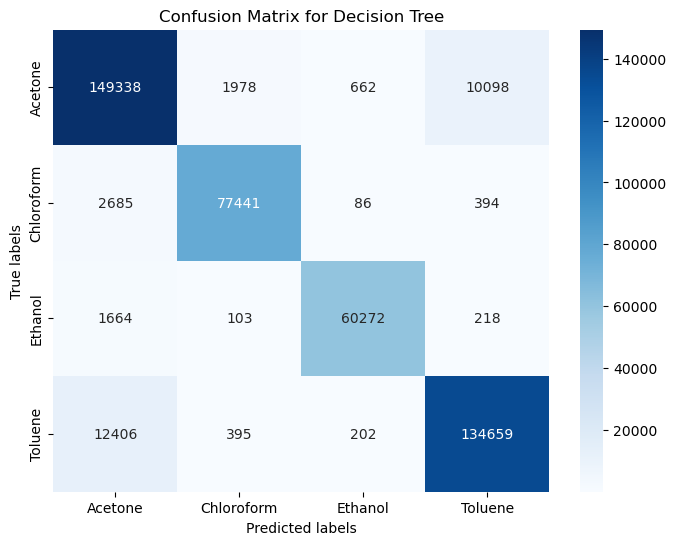
\includegraphics[width=0.8\linewidth]{Thesis Prashant//Images//Results/Confusion Decision.png}
    \caption{Confusion Matrix Decision Tree}
    \label{fig:enter-label}
\end{figure}

\subsection{Random Forest}
The Class of Decision Tree of arbitrary size has infinite VC dimension. So, a restriction on the size of the decision tree is needed. The danger of overfitting can be reduced by constructing an ensemble of trees. the method of $random forests$ was introduced by Breiman(2001). A random forest is a classifier consisting of a collection of a collection of decision trees, where each tree is constructed by applying an algorithm A on the training set S and an additional random vector, $\theta$, where, $\theta$ is sampled independent and identically distributed from distribution. A majority vote over the individual trees' predictions obtains the random forest's prediction.

\subsection{Random Forest Results}
A better model was obtained by Random Forest for all attributes that were converted to 0 to 1 as input and target variable hot encoded. The true negative, true positive, false negative, and false positive predictions for the entirely unknown data set of around four lac data points are explained in the confusion matrix.
\begin{figure}
    \centering
    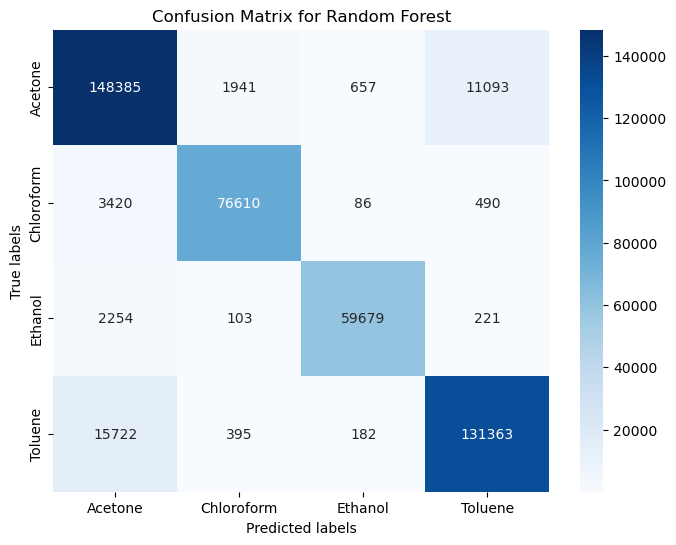
\includegraphics[width=0.8\linewidth]{Thesis Prashant//Images//Results/confusion_random_forest.png}
    \caption{Confusion Matrix Random Forest}
    \label{fig:enter-label}
\end{figure}